\documentclass[12pt,a4paper]{article}
\usepackage[utf8]{vietnam}
\usepackage{amsmath,amssymb}
\usepackage{geometry}
\geometry{top=1.5cm,bottom=1.2cm,left=1.4cm,right=1.4cm,headheight=28pt,headsep=12pt,footskip=18pt}
\usepackage{tikz}
\usepackage{xcolor}
\usepackage{enumerate}
\usepackage{graphicx}
\usepackage[version=4]{mhchem}
\usepackage{fancyhdr}
\usepackage{ex_test}

\renewcommand{\baselinestretch}{0.96}
\setlength{\parskip}{0pt}

\definecolor{hfRed}{RGB}{211,47,47}
\definecolor{hfGreen}{RGB}{139,195,144}

\pagestyle{fancy}
\fancyhf{}
\fancyhead[L]{\small\itshape\color{hfRed} Tài liệu lưu hành nội bộ}
\fancyhead[R]{\small\itshape\color{hfRed} Thầy \textbf{TRẦN VĂN THẠNH} - 0777.470.803}
\renewcommand{\headrulewidth}{0.8pt}
\renewcommand{\headrule}{\hbox to\headwidth{\color{hfGreen}\leaders\hrule height \headrulewidth\hfill}}

\fancyfoot[L]{\small\itshape\color{hfRed} CS1: 6/15 Nguyễn Hoàng, P. Kim Long, TP Huế \quad|\quad CS2: 24 Đặng Thái Thân, TP Huế}
\fancyfoot[R]{\small\bfseries\color{hfRed} Trang \thepage}
\renewcommand{\footrulewidth}{0.8pt}
\renewcommand{\footrule}{\hbox to\headwidth{\color{hfGreen}\leaders\hrule height \footrulewidth\hfill}}

\fancypagestyle{firstpage}{
  \fancyhf{}
  \renewcommand{\headrulewidth}{0pt}
  \fancyfoot[L]{\small\itshape\color{hfRed} CS1: 6/15 Nguyễn Hoàng, P. Kim Long, TP Huế \quad|\quad CS2: 24 Đặng Thái Thân, TP Huế}
  \fancyfoot[R]{\small\bfseries\color{hfRed} Trang \thepage}
  \renewcommand{\footrulewidth}{0.8pt}
  \renewcommand{\footrule}{\hbox to\headwidth{\color{hfGreen}\leaders\hrule height \footrulewidth\hfill}}
}

\begin{document}
\thispagestyle{firstpage}

\noindent
\begin{minipage}[t]{0.44\textwidth}
	\centering\fontsize{10pt}{12pt}\selectfont
	\textbf{SỞ GIÁO DỤC VÀ ĐÀO TẠO THỪA THIÊN HUẾ}\\
	\textbf{ĐỀ CHÍNH THỨC}\\
	\textit{(Đề thi có 04 trang)}
\end{minipage}\hfill
\begin{minipage}[t]{0.54\textwidth}
	\centering\small
	\textbf{ĐỀ KIỂM TRA ĐỊNH KỲ CHƯƠNG 2 (NITROGEN -- SULFUR)}\\
	\textbf{MÔN: HOÁ HỌC -- LỚP 11}\\
	\textit{Thời gian làm bài: 45 phút (không kể thời gian phát đề)}\\
	\fbox{\textbf{MÃ ĐỀ: 105}}
\end{minipage}

\smallskip
\noindent\hrulefill
\smallskip

\noindent\textbf{Họ, tên thí sinh:} \dotfill\ \textbf{Lớp:} \dotfill\ \textbf{Số báo danh:} \dotfill

\smallskip
\noindent\textit{(Cho biết nguyên tử khối: H = 1; C = 12; N = 14; O = 16; Na = 23; Mg = 24; Al = 27; S = 32; Cl = 35,5; Ar = 40; K = 39; Ca = 40; Fe = 56; Cu = 64; Zn = 65; Ba = 137).}
\smallskip

\noindent\textbf{\large PHẦN I. Câu trắc nghiệm nhiều phương án lựa chọn.}
\textit{Thí sinh trả lời từ câu 1 đến câu 18. Mỗi câu hỏi thí sinh chỉ chọn một phương án.}
\vspace{0.2cm}

\Opensolutionfile{ans}[ans-hoa11-de05hs]

\begin{ex}
Nguyên tố dinh dưỡng nào sau đây có trong cấu tạo của protein?
\choice
{Sắt}
{Kẽm}
{\True Nitrogen}
{Đồng}

\end{ex}

\begin{ex}
Để tạo độ xốp cho một số loại bánh, có thể dùng muối nào sau đây?
\choice
{$\ce{CaCO3}$}
{\True $\ce{NH4HCO3}$}
{$\ce{NH4Cl}$}
{$\ce{NaCl}$}

\end{ex}

\begin{ex}
Mưa acid ảnh hưởng tới hệ thực vật, phá hủy các vật liệu bằng kim loại, các bức tượng bằng đá, gây bệnh cho con người và động vật. Hiện tượng trên gây ra chủ yếu do khí thải của nhà máy nhiệt điện, phương tiện giao thông và sản xuất công nghiệp. Tác nhân chủ yếu trong khí thải gây ra mưa acid là
\begin{center}
	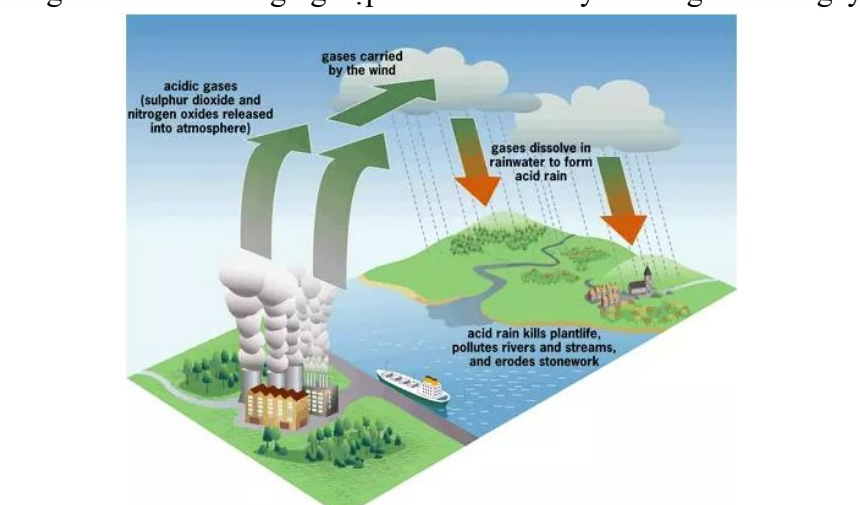
\includegraphics[width=0.62\textwidth]{images_crop_hoa11_de05/cau3_so_do_mua_acid.png}
\end{center}
\choice
{\True $\ce{SO2}$ và $\ce{NO2}$}
{$\ce{CH4}$ và $\ce{NH3}$}
{$\ce{CO}$ và $\ce{CH4}$}
{$\ce{CO}$ và $\ce{CO2}$}

\end{ex}

\begin{ex}
\textbf{(SBT - KNTT)} Oxide của nitrogen được tạo thành ở nhiệt độ cao, khi nitrogen có trong không khí bị oxi hóa được gọi là
\choice
{$\ce{NO_x}$ tức thời}
{\True $\ce{NO_x}$ nhiệt}
{$\ce{NO_x}$ nhiên liệu}
{$\ce{NO_x}$ tự nhiên}

\end{ex}

\begin{ex}
\textbf{(SBT - KNTT)} Công thức hoá học của diêm tiêu Chile là
\choice
{$\ce{Ca(NO3)2}$}
{$\ce{NH4NO3}$}
{$\ce{NH4Cl}$}
{\True $\ce{NaNO3}$}

\end{ex}

\begin{ex}
\textbf{(SBT - KNTT)} Sulfur đóng vai trò chất khử khi tác dụng với đơn chất nào sau đây?
\choice
{$\ce{Fe}$}
{\True $\ce{O2}$}
{$\ce{H2}$}
{$\ce{Hg}$}

\end{ex}

\begin{ex}
\textbf{(SBT - CTST)} Cách pha loãng dung dịch $\ce{H2SO4}$ đặc nào sau đây đúng?
\choice
{Rót nhanh acid vào nước và khuấy đều}
{Rót nhanh nước vào acid và khuấy đều}
{Rót từ từ nước vào acid và khuấy đều}
{\True Rót từ từ acid vào nước và khuấy đều}

\end{ex}

\begin{ex}
\textbf{(SBT - KNTT)} Trong nghiên cứu, khí nitrogen thường được dùng để tạo bầu khí quyển trơ dựa trên cơ sở nào?
\choice
{Nitrogen có tính oxi hoá mạnh}
{\True Nitrogen rất bền với nhiệt}
{Nitrogen khó hoá lỏng}
{Nitrogen không có cực}

\end{ex}

\begin{ex}
\textbf{(SBT - KNTT)} Xét cân bằng hóa học trong dung dịch nước:\\
$\ce{NH3 + H2O <=> NH4+ + OH-}$\\
Hằng số cân bằng ($K_\text{C}$) của phản ứng được biểu diễn bằng biểu thức nào sau đây?
\choice
{\True $K_\text{C} = \dfrac{[\ce{NH4+}][\ce{OH-}]}{[\ce{NH3}]}$}
{$K_\text{C} = \dfrac{[\ce{NH4+}][\ce{OH-}]}{[\ce{NH3}][\ce{H2O}]}$}
{$K_\text{C} = \dfrac{[\ce{NH4+}][\ce{OH-}]}{[\ce{H2O}]}$}
{$K_\text{C} = \dfrac{[\ce{NH4+}]}{[\ce{NH3}]}$}

\end{ex}

\begin{ex}
Trong các phản ứng dưới đây, phản ứng nào $\ce{NH3}$ \textbf{không} thể hiện tính khử?
\choice
{$\ce{4NH3 + 5O2 ->[xt, t^\circ] 4NO + 6H2O}$}
{\True $\ce{NH3 + HCl -> NH4Cl}$}
{$\ce{8NH3 + 3Cl2 -> 6NH4Cl + N2}$}
{$\ce{2NH3 + 3CuO ->[t^\circ] 3Cu + 3H2O + N2}$}

\end{ex}

\begin{ex}
Thí nghiệm với dung dịch $\ce{HNO3}$ thường sinh ra khí độc $\ce{NO2}$. Để hạn chế khí $\ce{NO2}$ thoát ra từ ống nghiệm, người ta nút ống nghiệm bằng:
\begin{enumerate}[(a)]
	\item bông khô.
	\item bông có tẩm nước.
	\item bông có tẩm nước vôi.
	\item bông có tẩm giấm ăn.
\end{enumerate}
Trong 4 biện pháp trên, biện pháp có hiệu quả nhất là
\choice
{(d)}
{\True (c)}
{(a)}
{(b)}

\end{ex}

\begin{ex}
Ứng dụng nào sau đây \textbf{không} phải của $\ce{SO2}$?
\choice
{Sản xuất sulfuric acid}
{Tẩy màu dung dịch đường}
{\True Khử mùi không khí}
{Tẩy trắng giấy, bột giấy}

\end{ex}

\begin{ex}
Trong điều kiện thích hợp, xảy ra các phản ứng sau:
\begin{enumerate}[(a)]
	\item $\ce{2H2SO4 + C -> 2SO2 + CO2 + 2H2O}$
	\item $\ce{H2SO4 + Fe(OH)2 -> FeSO4 + 2H2O}$
	\item $\ce{4H2SO4 + 2FeO -> Fe2(SO4)3 + SO2 + 4H2O}$
	\item $\ce{6H2SO4 + 2Fe -> Fe2(SO4)3 + 3SO2 + 6H2O}$
\end{enumerate}
Trong các phản ứng trên, phản ứng xảy ra với dung dịch $\ce{H2SO4}$ loãng là
\choice
{(a)}
{(c)}
{\True (b)}
{(d)}

\end{ex}

\begin{ex}
Dẫn khí $\ce{SO2}$ vào dung dịch $\ce{KMnO4}$ hiện tượng quan sát được là
\choice
{Dung dịch không màu chuyển sang màu tím}
{Dung dịch màu tím bị vẩn đục màu vàng}
{Màu tím của dung dịch $\ce{KMnO4}$ chuyển sang màu vàng}
{\True Màu tím của dung dịch $\ce{KMnO4}$ chuyển sang không màu}

\end{ex}

\begin{ex}
Nguyên nhân chủ yếu gây ra hiện tượng phú dưỡng trong các thủy vực là gì?
\choice
{Sự tích tụ các chất hữu cơ do phân hủy xác sinh vật}
{\True Sự gia tăng quá mức các chất dinh dưỡng như nitrate ($\ce{NO3-}$) và phosphate ($\ce{PO4^3-}$) từ nước thải sinh hoạt, phân bón nông nghiệp và công nghiệp}
{Sự thay đổi nhiệt độ nước trong thủy vực}
{Quá trình xói mòn đất làm thay đổi hệ sinh thái nước ngọt}

\end{ex}

\begin{ex}
Mưa acid có thể gây ra tác động tiêu cực nào đối với các công trình xây dựng?
\choice
{Làm tăng độ bền của các công trình xây dựng bằng đá vôi}
{\True Gây ăn mòn các công trình làm từ đá vôi, đá cẩm thạch và kim loại}
{Tăng khả năng chống chịu của các vật liệu xây dựng trước sự tác động của môi trường}
{Không có tác động đến các công trình xây dựng}

\end{ex}

\begin{ex}
Biện pháp nào dưới đây có thể giúp giảm thiểu hiện tượng mưa acid?
\choice
{Tăng cường việc sử dụng các loại nhiên liệu hóa thạch}
{\True Giảm lượng khí thải $\ce{SO2}$ và $\ce{NO_x}$ từ các nhà máy công nghiệp và phương tiện giao thông}
{Sử dụng nhiều hơn các loại phân bón chứa phosphate}
{Khuyến khích việc phát triển giao thông đường bộ}

\end{ex}

\begin{ex}
Cho các phát biểu sau:
\begin{enumerate}[(1)]
	\item Cho thanh Fe (iron) vào dung dịch $\ce{H2SO4}$ loãng, iron tan ra, sủi bọt khí.
	\item Cho dung dịch $\ce{BaCl2}$ vào dung dịch $\ce{H2SO4}$, xuất hiện kết tủa đen.
	\item Ở nhiệt độ cao, sulfur tác dụng với hydrogen tạo thành hydrogen sulfide ($\ce{H2S}$).
	\item Cho từng giọt sulfuric acid đặc vào đường saccharose ($\ce{C12H22O11}$) màu trắng, đường chuyển màu nâu $\rightarrow$ đen sau đó trào lên khỏi miệng cốc.
	\item Nitrogen lỏng được dùng để làm lạnh nhanh, bảo quản mẫu vật phẩm trong y học.
	\item Nitrogen bền nhiệt, có tính trơ nên không bảo quản được hương vị thực phẩm.
	\item Không khí có chứa oxygen là tác nhân oxi hóa thực phẩm, làm thực phẩm ôi thiu chậm hơn trong khí nitrogen.
\end{enumerate}
Số phát biểu đúng là
\choice
{3}
{\True 4}
{5}
{6}

\end{ex}

\Closesolutionfile{ans}

\vspace{0.3cm}
\noindent\textbf{\large PHẦN II. Câu trắc nghiệm đúng sai.}
\textit{Thí sinh trả lời từ câu 1 đến câu 4. Trong mỗi ý a), b), c), d) ở mỗi câu, thí sinh chọn đúng hoặc sai.}
\vspace{0.2cm}

\begin{ex}
Để giảm sốt hoặc giảm đau, người ta có thể dùng túi chườm lạnh chứa hóa chất. Hãy tìm hiểu về loại túi chườm lạnh này:
\begin{center}
	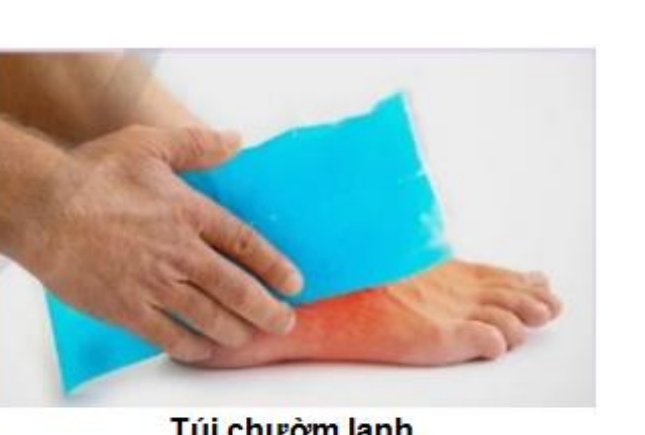
\includegraphics[width=0.45\textwidth]{images_crop_hoa11_de05/cau1_p2_tui_chuom_lanh.png}
\end{center}
\choiceTF
{\True Hóa chất trong túi chườm lạnh gồm ammonium chloride rắn và nước cất}
{\True Túi chườm sẽ hoạt động khi phá vỡ lớp ngăn cách giữa muối ammonium chloride và nước cất}
{Do sự hòa tan $\ce{NH4Cl(s)}$ vào nước là một quá trình tỏa nhiệt: $\ce{NH4Cl(s) -> NH4Cl(aq)}\ \Delta_r H^\circ_{298} < 0$}
{Phản ứng tỏa nhiệt, muối hấp thụ nhiệt từ nước, làm nước giảm nhiệt độ}

\end{ex}

\begin{ex}
Biện pháp nào sau đây dùng để hạn chế hiện tượng phú dưỡng?
\choiceTF
{\True Tạo điều kiện để nước trong kênh rạch, ao, hồ được lưu thông}
{Xả nước thải (nông nghiệp, công nghiệp và sinh hoạt) trực tiếp đến ao, hồ thông qua các cống dẫn nước cố định}
{\True Sử dụng phân bón đúng liều lượng, đúng cách, đúng thời điểm trong năm để hạn chế sự rửa trôi của ion nitrate và phosphate từ nguồn phân bón dư thừa vào kênh rạch, ao, hồ}
{\True Xử lí nước thải trước khi cho vào kênh rạch, ao, hồ}

\end{ex}

\begin{ex}
Với lứa tuổi học sinh có thể giúp giảm thiểu lượng sulfur dioxide thải vào không khí bằng các việc làm phù hợp:
\choiceTF
{\True Khuyến khích sử dụng xe điện, sử dụng nguyên liệu thân thiện môi trường như xăng E5,...}
{Khuyến khích đốt rác thải}
{\True Tuyên truyền tác hại của $\ce{SO2}$ và lợi ích của nhiên liệu tái tạo, bảo vệ môi trường,...}
{\True Giảm rác thải, phân loại rác, tái chế, tái sử dụng}

\end{ex}

\begin{ex}
Sulfuric acid có tính acid, tính oxi hóa mạnh, tính háo nước:
\choiceTF
{\True Sulfuric acid đặc phản ứng với carbon trong than}
{\True Sulfuric acid đặc oxi hoá hợp chất Fe(II) thành hợp chất Fe(III)}
{Cho bột sodium hydrogencarbonate vào sulfuric acid loãng xuất hiện kết tủa trắng}
{\True Chất rắn copper (II) sulfate pentahydrate có màu xanh tác dụng với sulfuric acid đặc sẽ biến thành copper (II) sulfate khan màu trắng}

\end{ex}

\vspace{0.3cm}
\noindent\textbf{\large PHẦN III. Câu trắc nghiệm yêu cầu trả lời ngắn.}
\textit{Thí sinh trả lời từ câu 1 đến câu 6.}
\vspace{0.2cm}

\begin{ex}
Phú dưỡng là hệ quả sau khi ao ngòi, sông hồ nhận quá nhiều các nguồn thải chứa các chất dinh dưỡng chứa nguyên tố nitrogen, phosphorus. Khi hàm lượng phosphorus vượt quá $20\ \mu\text{g/L}$ và hàm lượng nitrogen vượt quá ngưỡng bao nhiêu $\mu\text{g/L}$ thì xảy ra hiện tượng phú dưỡng?

\vspace{1.0cm}

\end{ex}

\begin{ex}
Cho các chất khí sau: $\ce{H2S, NO, NO2, SO2}$. Số khí gây ô nhiễm môi trường khi phát thải vào không khí là bao nhiêu?

\vspace{1.0cm}

\end{ex}

\begin{ex}
\textbf{(SBT - KNTT)} Tính khối lượng riêng (g/L) của không khí ở điều kiện chuẩn, giả thiết thành phần không khí gồm: 78\% nitrogen, 21\% oxygen và 1\% argon (làm tròn kết quả đến hàng phần trăm).

\vspace{1.5cm}

\end{ex}

\begin{ex}
Trong công nghiệp, ammonia được sản xuất theo phản ứng pha khí:
\[\ce{N2(g) + 3H2(g) <=> 2NH3(g)} \quad \Delta_r H^\circ_{298}\]
Cho biết các giá trị năng lượng liên kết $E_\text{b}\ (\text{kJ}\cdot\text{mol}^{-1})$:
\begin{center}
\begin{tabular}{|c|c|c|c|}
\hline
\textbf{Liên kết} & $\ce{N\bond{3}N}$ & $\ce{H-H}$ & $\ce{N-H}$ \\ \hline
$E_\text{b}$ & 945 & 436 & 386 \\ \hline
\end{tabular}
\end{center}
Nhiệt tạo thành $\Delta_f H^\circ_{298}\ (\text{kJ}\cdot\text{mol}^{-1})$ của $\ce{NH3(g)}$ là $-x\text{ kJ}\cdot\text{mol}^{-1}$. Giá trị của $x$ là bao nhiêu?

\vspace{1.5cm}

\end{ex}

\begin{ex}
Sự phụ thuộc của độ tan khí ammonia trong nước vào nhiệt độ được mô tả ở hình bên.
\begin{center}
	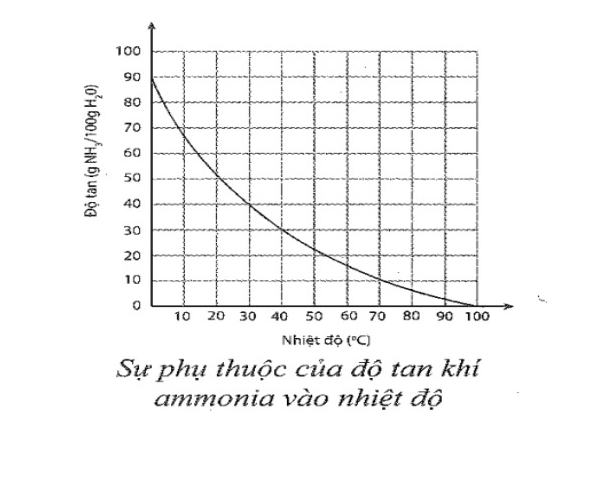
\includegraphics[width=0.48\textwidth]{images_crop_hoa11_de05/cau5_p3_do_thi_do_tan_nh3.png}
\end{center}
Dựa vào đồ thị ở hình bên, hãy xác định: Nồng độ phần trăm của dung dịch ammonia bão hòa ở $30^\circ\text{C}$ (làm tròn kết quả đến hàng phần mười).

\vspace{1.5cm}

\end{ex}

\begin{ex}
Sau hiện tượng phú dưỡng, một hồ nước có diện tích bề mặt $1\text{ km}^2$ và độ sâu trung bình $5\text{ m}$ chứa một lượng lớn xác tảo. Lượng oxygen hòa tan (DO) ban đầu trong hồ là $8\text{ mg/L}$, nhưng sau quá trình phân hủy xác tảo, nồng độ oxygen giảm xuống còn $2\text{ mg/L}$. Lượng oxygen (tính bằng kg) đã bị tiêu thụ trong toàn bộ hồ là $x$ nghìn kg. Tính giá trị $x$?

\vspace{1.5cm}

\end{ex}

\vspace{0.3cm}
\noindent\textbf{\large PHẦN IV. Tự luận}
\textit{Học sinh giải chi tiết các câu hỏi sau vào giấy làm bài.}
\vspace{0.2cm}

\begin{ex}
\textbf{[CĐ - SGK]} Viết phương trình hóa học minh họa tác động của mưa acid đối với calcium carbonate trong núi đá vôi và với kim loại iron có trong thép.

\vspace{2.5cm}

\end{ex}

\begin{ex}
\textbf{(SBT - KNTT)} Trong công nghiệp, ammonia được sản xuất theo phản ứng pha khí:
\[\ce{N2(g) + 3H2(g) <=> 2NH3(g)} \quad \Delta_r H^\circ_{298}\]
Cho biết các giá trị năng lượng liên kết $E_\text{b}\ (\text{kJ}\cdot\text{mol}^{-1})$:
\begin{center}
\begin{tabular}{|c|c|c|c|}
\hline
\textbf{Liên kết} & $\ce{N\bond{3}N}$ & $\ce{H-H}$ & $\ce{N-H}$ \\ \hline
$E_\text{b}$ & 945 & 436 & 386 \\ \hline
\end{tabular}
\end{center}
a) Tính nhiệt phản ứng $\Delta_r H^\circ_{298}$ của phản ứng ở điều kiện chuẩn, nhận xét về dấu và độ lớn của giá trị tìm được.\\
b) Tính nhiệt tạo thành $\Delta_f H^\circ_{298}\ (\text{kJ}\cdot\text{mol}^{-1})$ của $\ce{NH3(k)}$.

\vspace{3.5cm}

\end{ex}

\begin{center}
\textbf{--------- HẾT ---------}
\end{center}

\end{document}
